
\begin{table}
	\caption{Association between the variables' instantiation (\textup{\textbf{Candidate}}) to the data associating it (\textup{\textbf{Knowledge Base Facts}}).}
	\begin{tabular}{lp{0.38\textwidth}}
		\toprule
		\textbf{Candidate} & \textbf{Knowledge Base Facts}\\
		\midrule
		Rome & Abigail came back to Rome.\\
		Rome & On September 1988, Abigail moved from Bologna's to La Sapienza University, Rome.\\
		Latium & Yesterday (2018/06/22) Abigail was seen in Latium.\\
		Turin & Abigail was rushed to the ``Umberto I'' hospital in Turin.\\
		Minneapolis & Abigail did a trip to Minneapolis on 1987.\\
		Duluth & Then, Abigail travelled from Minneapolis to Dulduth.\\
		\bottomrule
	\end{tabular}
	\label{tab:datahyp}
\end{table} \begin{figure} 
	\centering
	\subfloat[``\textit{Where did Abigail go?}'']{%
		\label{subfig:q1}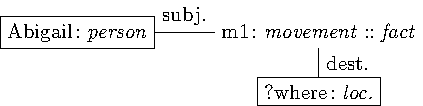
\includegraphics[width=.5\linewidth]{fig/question01.pdf}}
	\hfill
	\subfloat[``\textit{In which places did Calbert not go?}'']{\label{subfig:q4}
		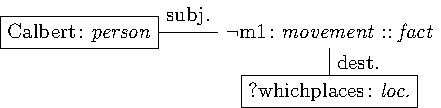
\includegraphics[width=0.45\linewidth]{fig/question04.pdf}}
	\\
	\subfloat[``\textit{Which crimes did Bradford committed before going to jail?}'']{%
		\label{subfig:q2}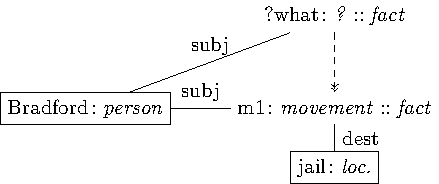
\includegraphics[width=.5\linewidth]{fig/question02.pdf}}
	\hfill
	\subfloat[``\textit{Who robbed the bank before travelling to Paris?}'']{%
		\label{subfig:q2b}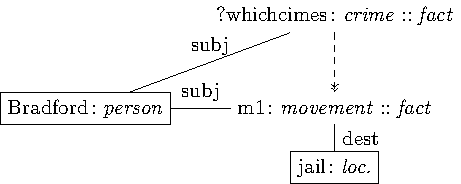
\includegraphics[width=.5\linewidth]{fig/question02bis.pdf}}\\
	\subfloat[``\textit{Which crimes did Bradford committed before going to jail?}'']{%
		\label{subfig:q3}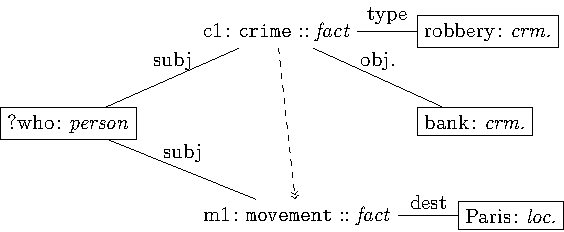
\includegraphics[width=.7\linewidth]{fig/question03.pdf}}\\
	\subfloat[``\textit{Which crime was committed by the person that first travelled to Paris?}'']{%
		\label{subfig:q3b}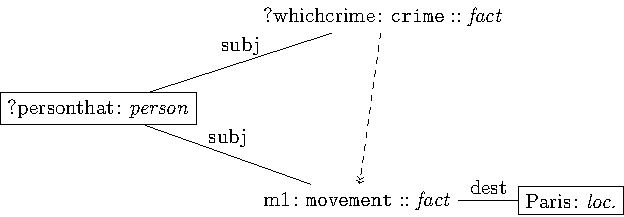
\includegraphics[width=.7\linewidth]{fig/question03b.pdf}}
	\caption{Each entity/filler is represented by a rectangle, facts have no shape and fact's fields are represented by straight edges. Variables are represented by names preceded by a question mark, ?. Temporal associations between facts are represented by dashed edges.}
	\label{fig:querygraph} 
\end{figure}


\section{Query Interpretation}\label{sec:querinterp}
Given that (natural language) queries can be expressed either as a declarative language \cite{Li16,Saha16} or using the same format as the data \cite{Hu0YWZ18,Consens90} (e.g., graphs), this paper uses the latter approach because its representation is language independent. Moreover, the latter approach is also able to express most of the natural language queries of interest within our scenario \texttt{[TODO]}. 

With reference to Figure \ref{fig:querygraph}, each entity and filler can be expressed as a vertex, while each binary relationship can be expressed as a edge, and facts can be expressed as hyperedges connecting different vertices \cite{Fagin83}. Negations can be expressed by juxtaposing the $\neg$ symbol. Natural language uses adverbs or pronouns to identify which are the elements to be returned by the query, namely \textit{variables}, which are represented as nodes (or edges) which name starts with a question mark.  Such variable instantiation can be performed by approximate graph matching the query graph to the data represented in the knowledge base \cite{DeVirgilio2015}, thus creating a set of \textit{morphisms} linking each variable to the corresponding matched KB elements (\textit{candidate}). The KB's subgraph containing all the candidates for a given morphism is an \textit{hypothesis} $h$.  E.g., Table \ref{tab:datahyp} provides in its left column a set of possible hypotheses' candidates generated from the knowledge base data and answering the query ``\textit{Where did Abigail go?}'. 

We now analyse four possible queries of interest within our scenario \texttt{[TODO]}:

\begin{enumerate}
\item \textbf{Return an entity or filler associated to a given fact or relationship.} E.g., for ``\textit{Where did Abigail go?}'' (Figure \ref{subfig:q1}), \textit{go} is the keyword identifying the fact for the specific \texttt{movement} type, while \textit{where} identifies the element to be returned and its type, that is a \textit{location}. Therefore, the query asks for all the facts expressing a movement (\textit{go}) of Abigail towards a specific location (\textit{where}). 
\item \textbf{Return a fact associated to a given fact or relationship.} E.g., in ``\textit{What did Bradford do before going to jail?}'' (Figure \ref{subfig:q2}), the keywords \textit{What} and \textit{do} specify that we need to return a fact which is liked via a temporal association (\textit{before}) to another fact or relationship (\textit{Bradford \dots going to jail}). In this case, the to-be-returned fact may have any possible type. The same question can be also refined to return a specific fact type as in the former example: e.g., ``\textit{Which crimes did Bradford committed before going to jail?}'' (Figure \ref{subfig:q2b}) may specify to return all the facts pertaining to Bradford's criminal record.
\item \textbf{Variables appearing in multiple facts/relationships.} E.g., ``\textit{Who robbed the bank before travelling to Paris?}'' (Figure \ref{subfig:q3}) asks to return an entity (\textit{Who}) which first appears in a \texttt{movement} fact (\textit{Who \dots travelling to Paris}) and, later on, performed a \texttt{crime} (\textit{Who robbed the bank}). We want to return an entity  appearing in two distinct events having a temporal association. This corresponds to a join between two facts where the criminal corresponds to a moving person. 

We can rephrase the same query to return a fact having a variable binding as follows: \textit{Which crime was committed by the person that first travelled to Paris?} (Figure \ref{subfig:q3b}). In this case the variable binding is made explicit by the keywords \textit{person} and \textit{that}, while \textit{Which} remarks that we now want to return only the criminal facts.
\item \textbf{Negated queries.} E.g., for ``\textit{In which places did Calbert not go?}'' (Figure \ref{subfig:q4}), we can provide either all the \textit{places} appearing in negated place relationships or \texttt{movement} facts, or return a set of all the possible \textit{places} not appearing in non-negated \texttt{place} relationships and \texttt{movement} facts.  Please note that such queries can be directly expressed in graph query languages which, on the other hand, do not usually query data that may contain negations. On the other hand, current graph pattern matching frameworks may only express positive facts.
\end{enumerate}

